The runtime view of the software is described by a set of UML sequence diagrams that shows how the software will behave.\\
Note that the processes of registration and login are analyzed only for users but they are very similar for third parties.

\begin{figure}[h!]
	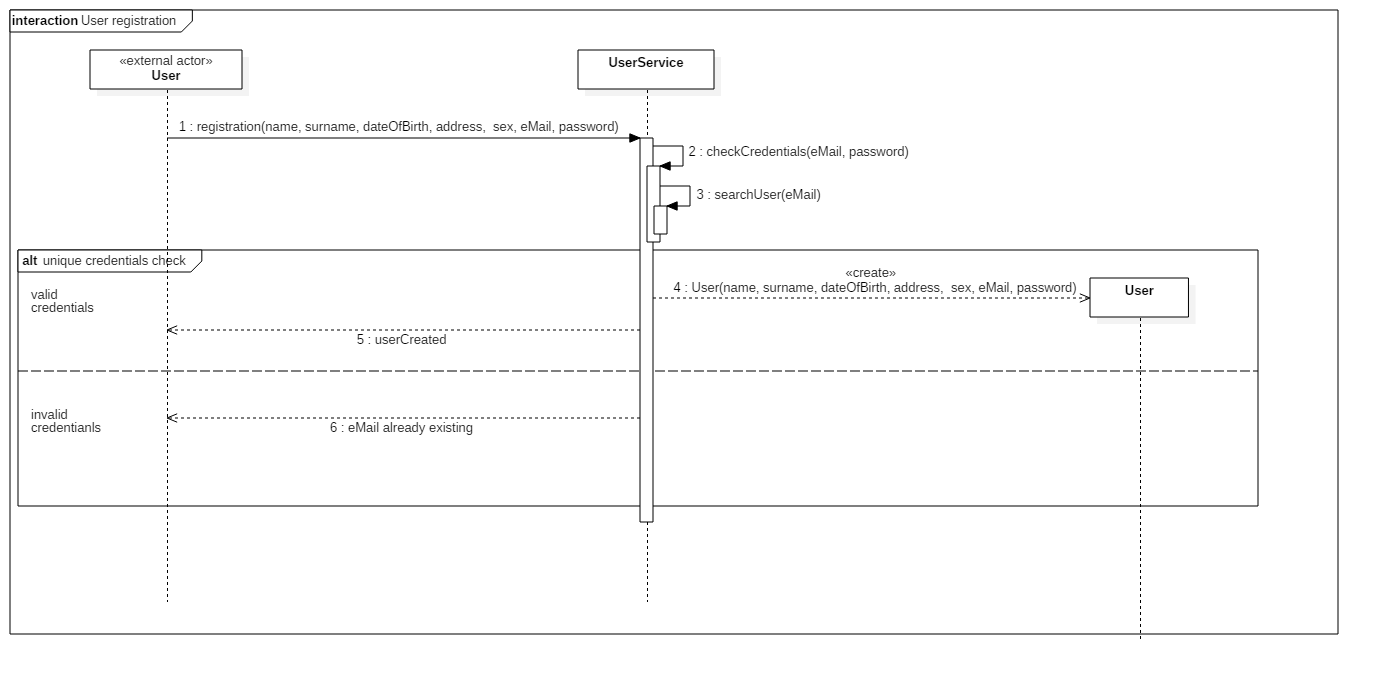
\includegraphics[width=1.0\textwidth]{./pictures/sequence_userRegistration.png}\par
	\caption{Sequence diagram about the registration of a user.}
\end{figure}
\FloatBarrier 

\begin{figure}[h!]
	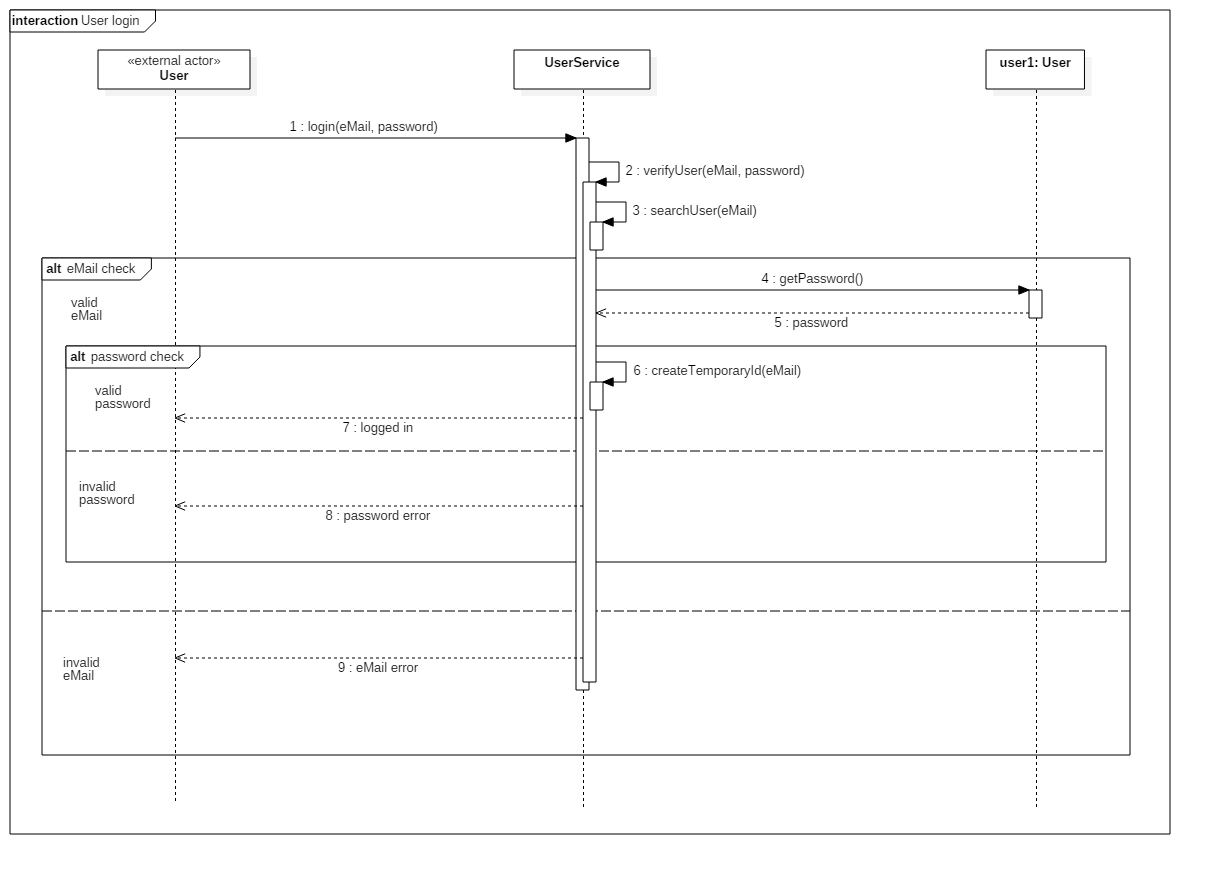
\includegraphics[width=1.0\textwidth]{./pictures/sequence_userLogin.png}\par
	\caption{Sequence diagram about the login of a user.}
\end{figure}
\FloatBarrier 

\begin{figure}[h!]
	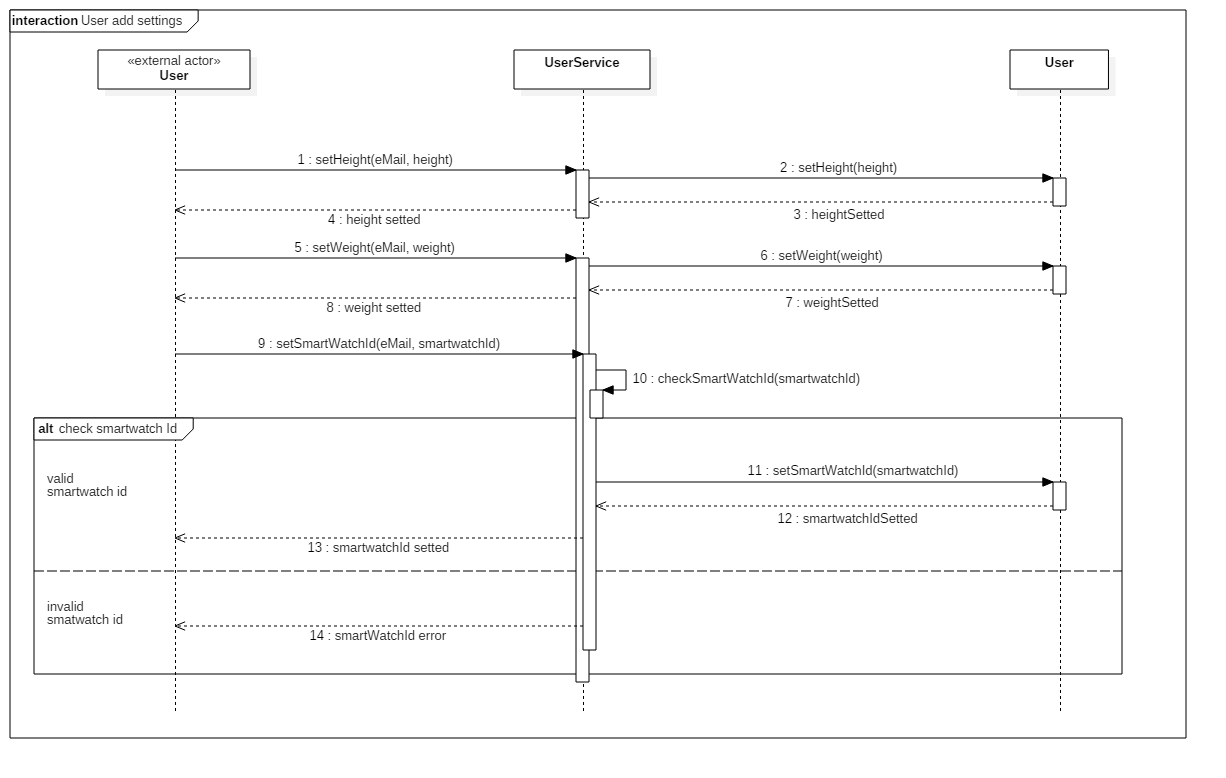
\includegraphics[width=1.0\textwidth]{./pictures/sequence_userSettings.png}\par
	\caption{Sequence diagram about adding a user's settings.}
\end{figure}
\FloatBarrier 

\begin{figure}[h!]
	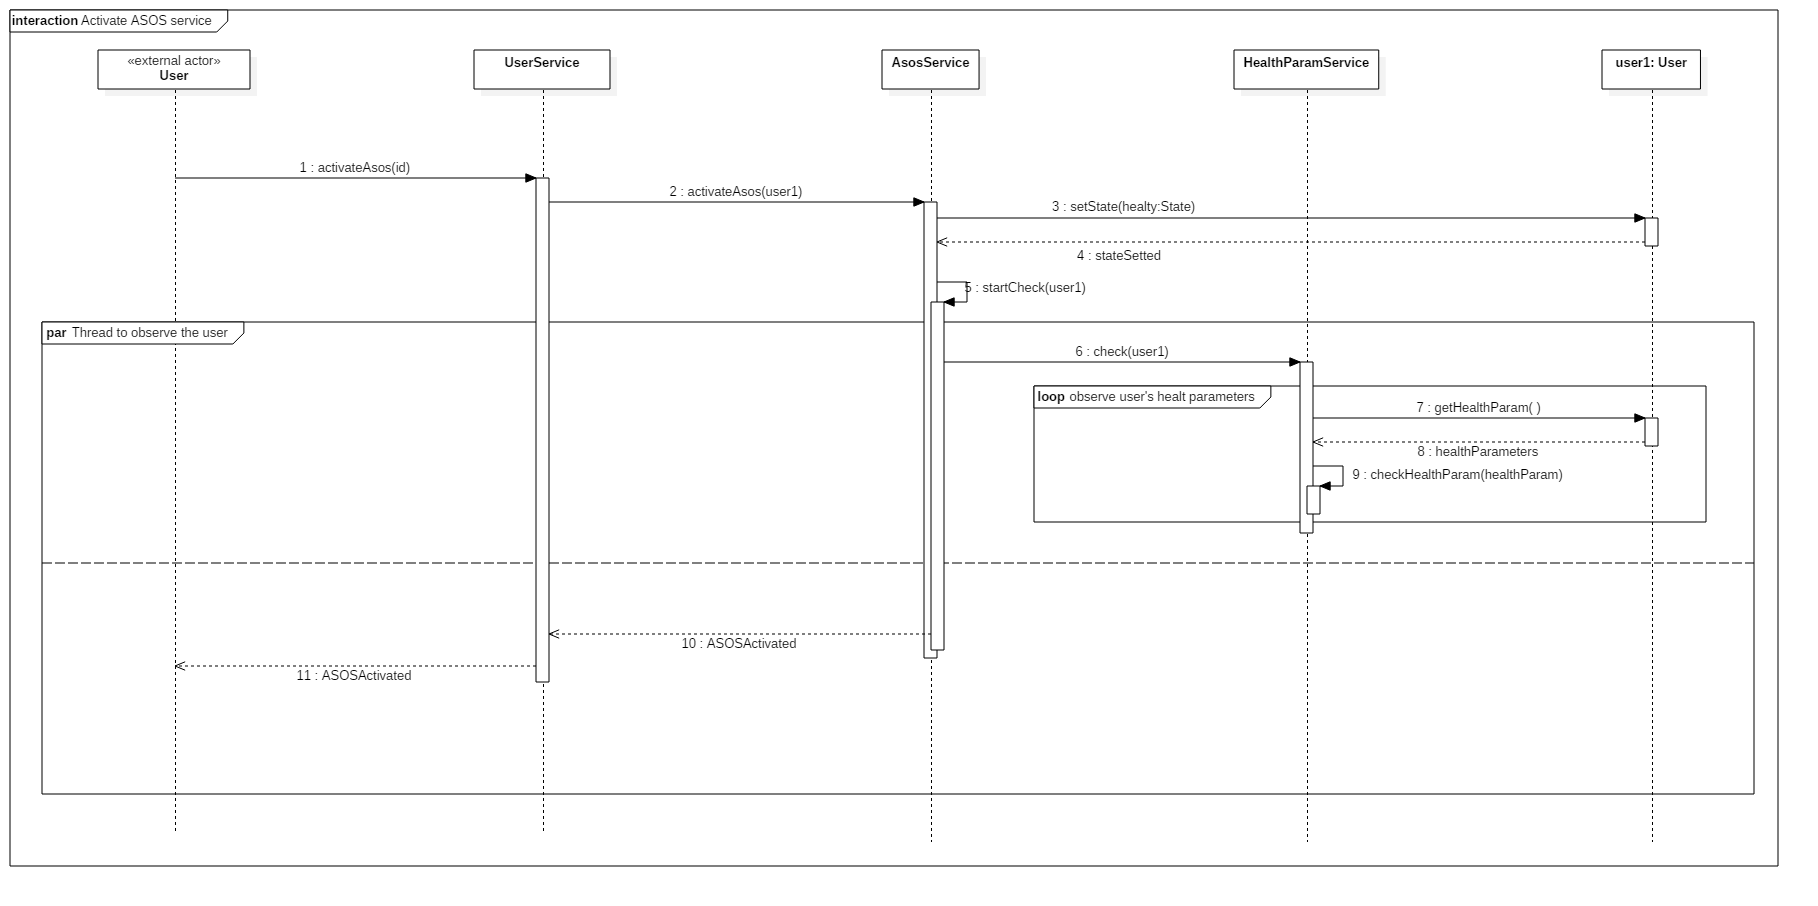
\includegraphics[width=1.0\textwidth]{./pictures/sequence_activateAsos.png}\par
	\caption{Sequence diagram about the activation of ASOS.}
\end{figure}
\FloatBarrier 

\begin{figure}[h!]
	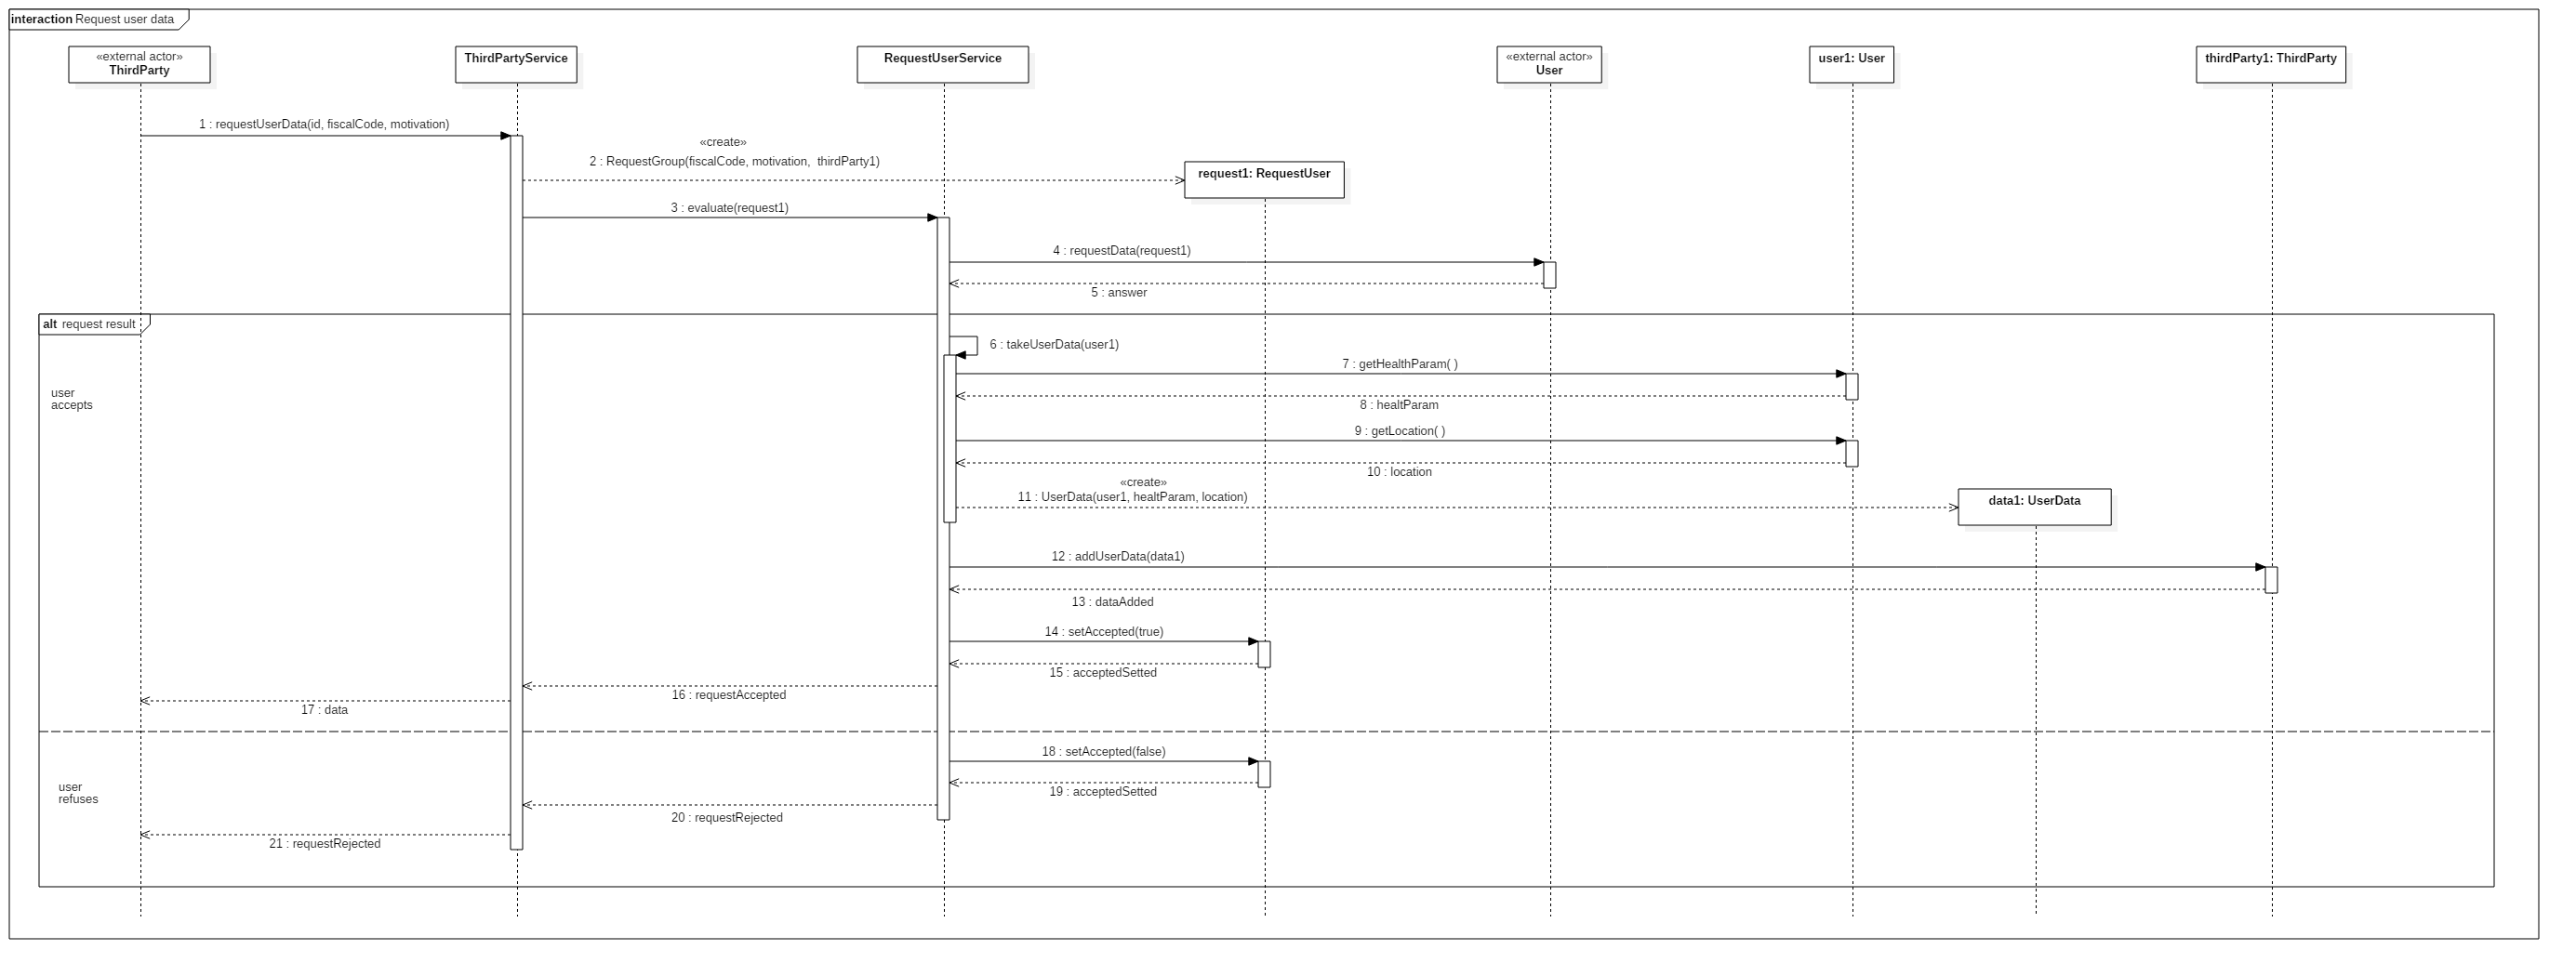
\includegraphics[width=1.0\textwidth]{./pictures/sequence_userRequest.png}\par
	\caption{Sequence diagram about requesting data about a user.}
\end{figure}
\FloatBarrier 

\begin{figure}[h!]
	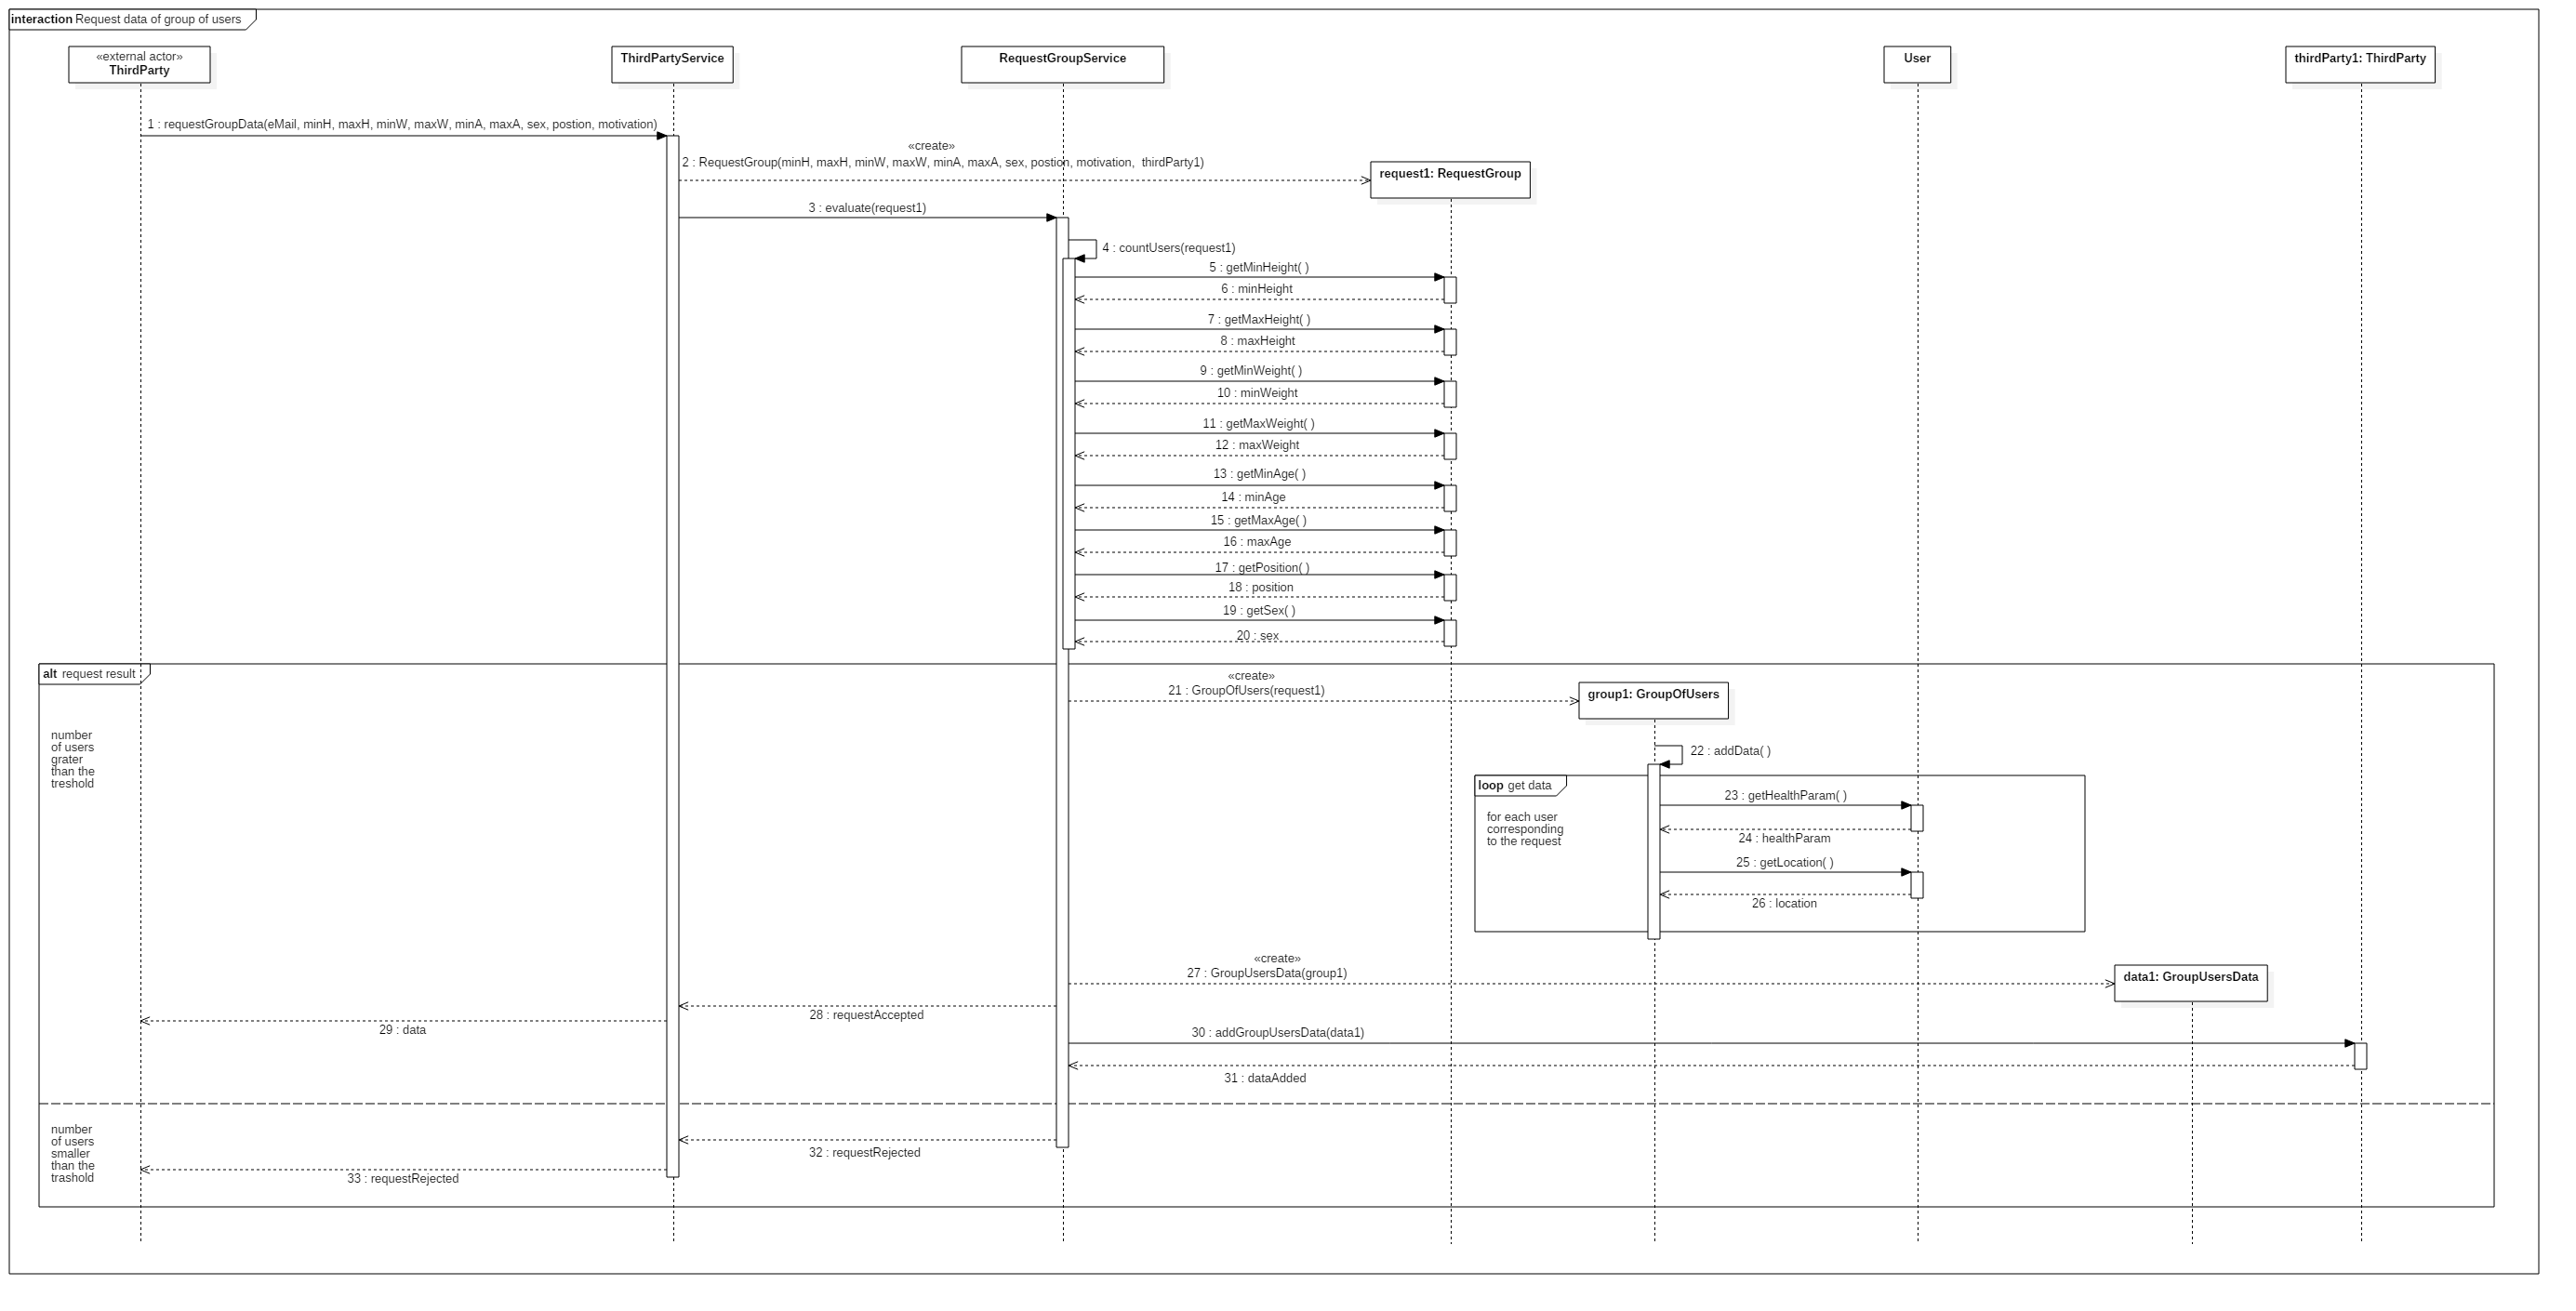
\includegraphics[width=1.0\textwidth]{./pictures/sequence_groupRequest.png}\par
	\caption{Sequence diagram about requesting data about a group of users.}
\end{figure}
\FloatBarrier 

\begin{figure}[h!]
	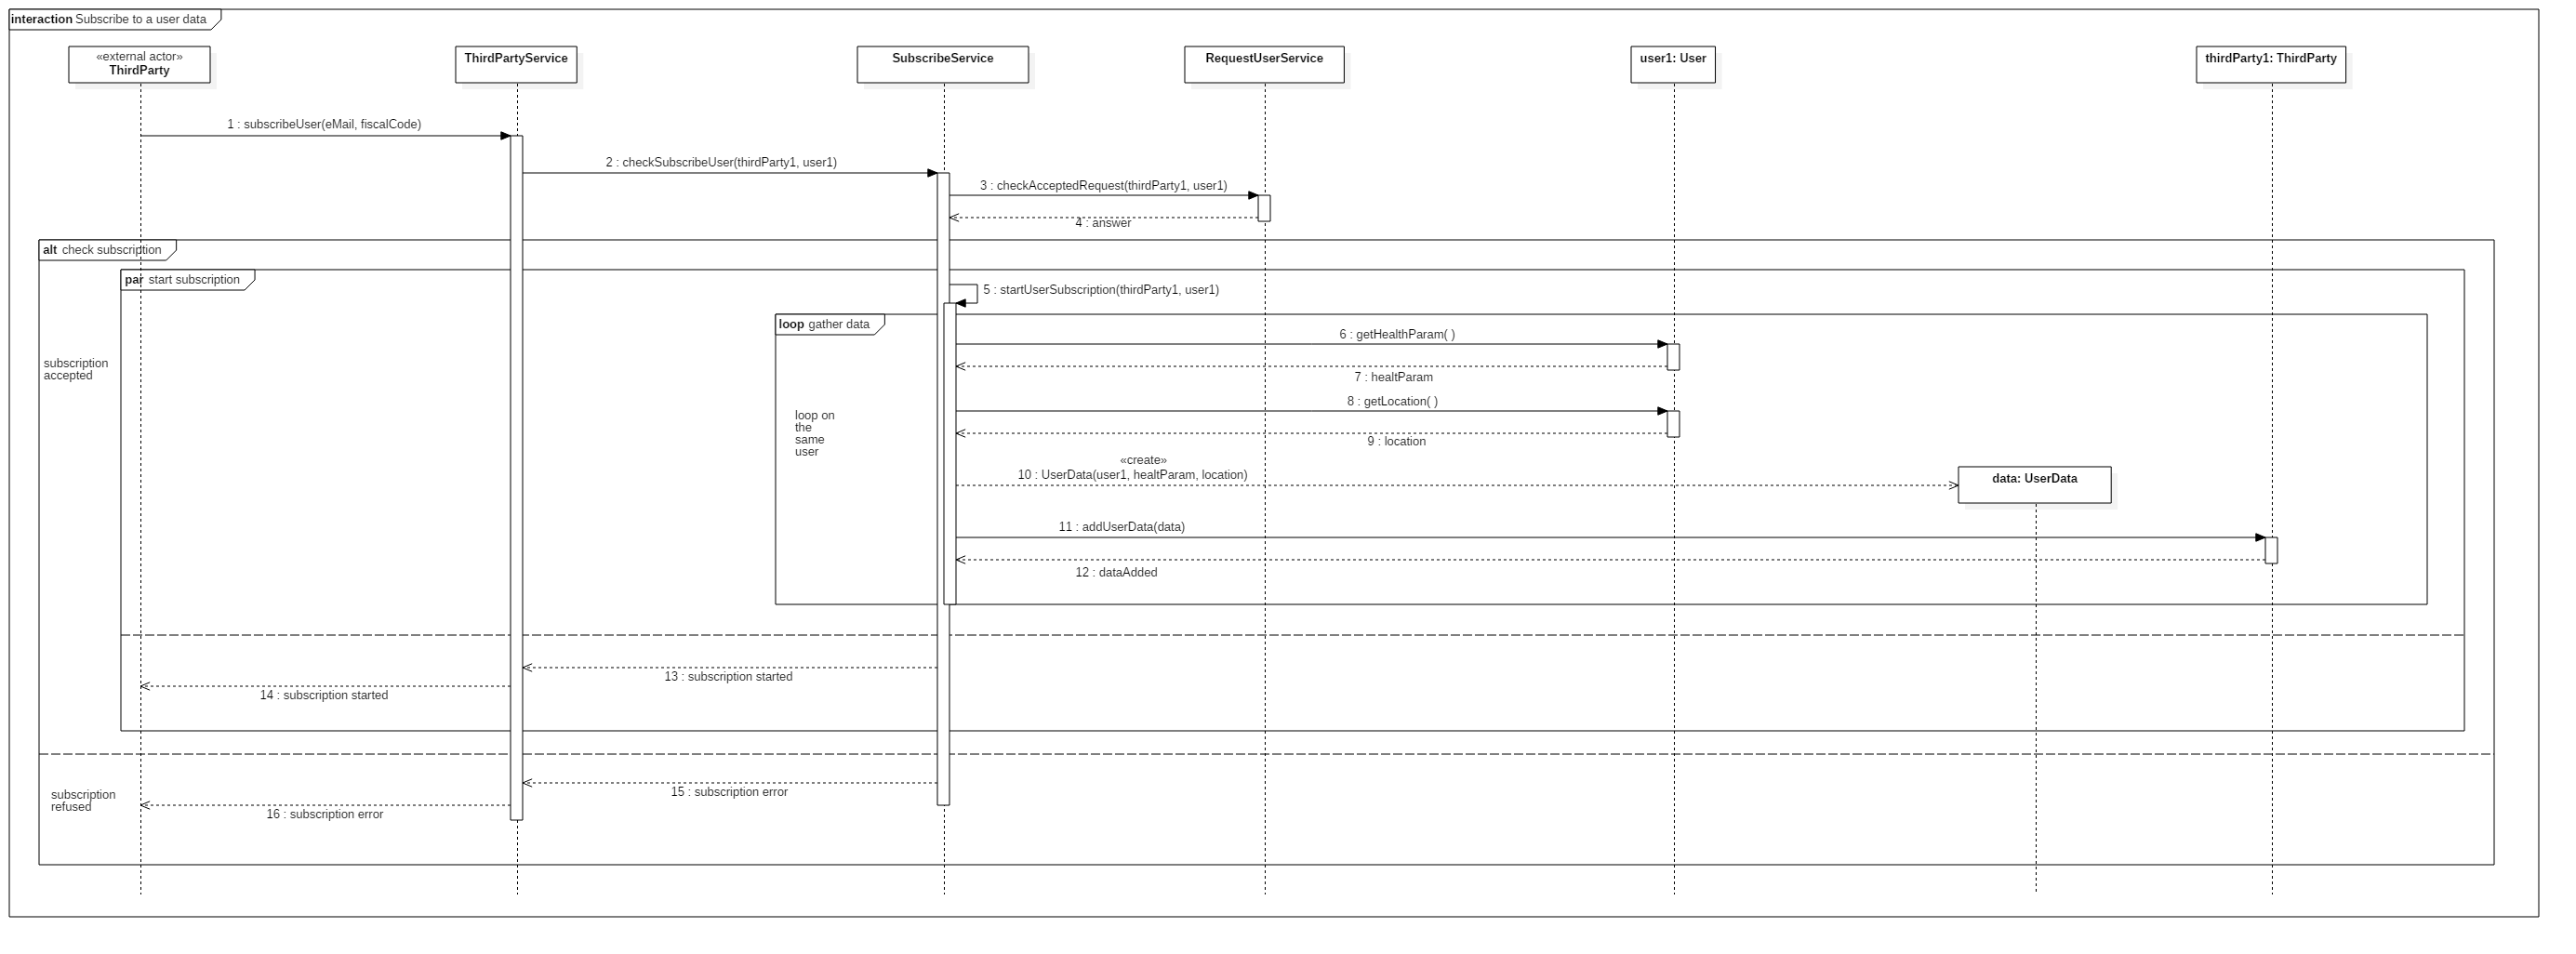
\includegraphics[width=1.0\textwidth]{./pictures/sequence_userSubscribe.png}\par
	\caption{Sequence diagram about subscribing to a user data.}
\end{figure}
\FloatBarrier 

\begin{figure}[h!]
	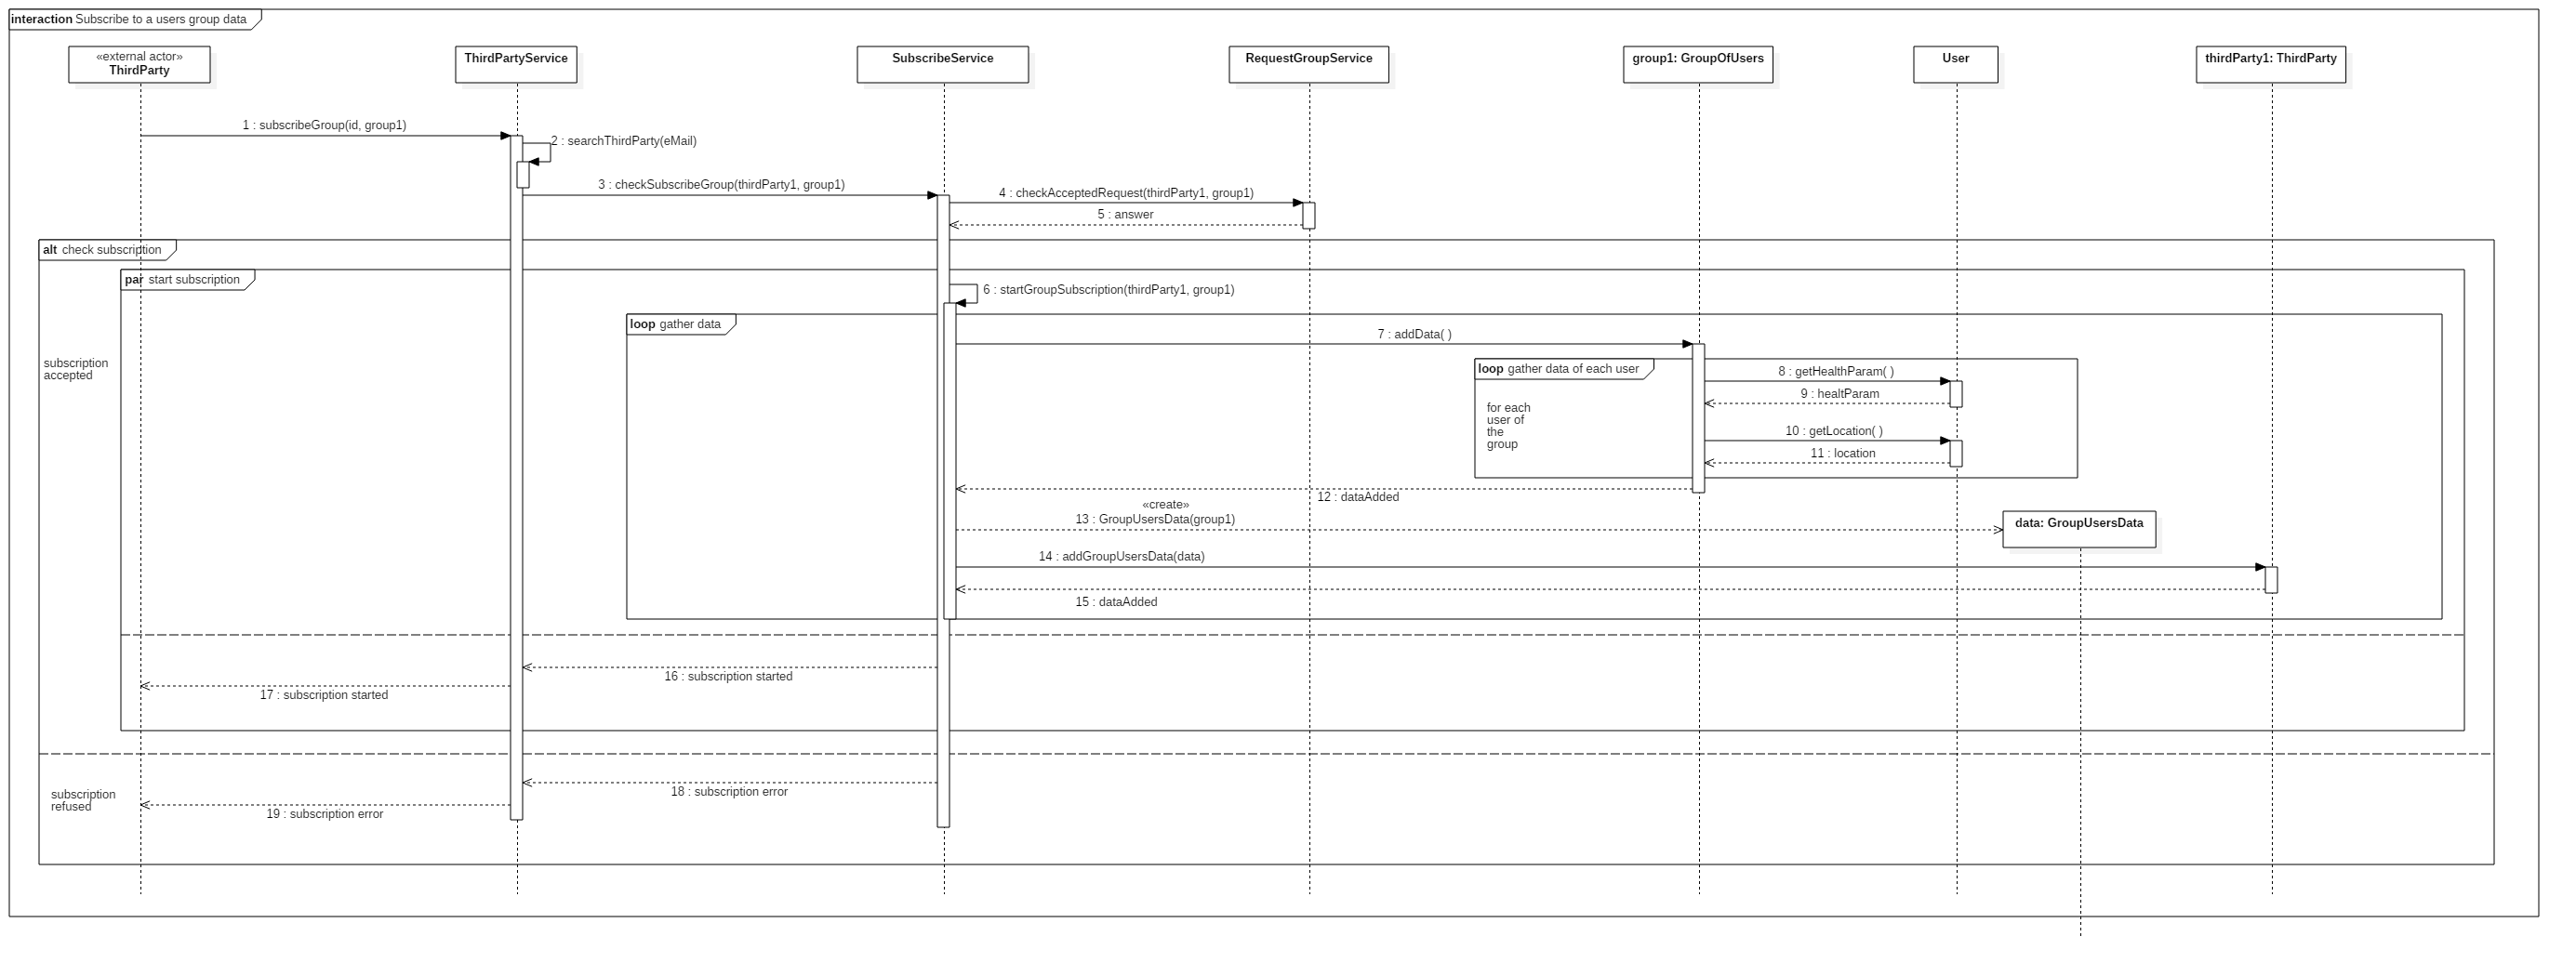
\includegraphics[width=1.0\textwidth]{./pictures/sequence_groupSubscribe.png}\par
	\caption{Sequence diagram about subscribing to a users group data.}
\end{figure}
\FloatBarrier 

\begin{figure}[h!]
	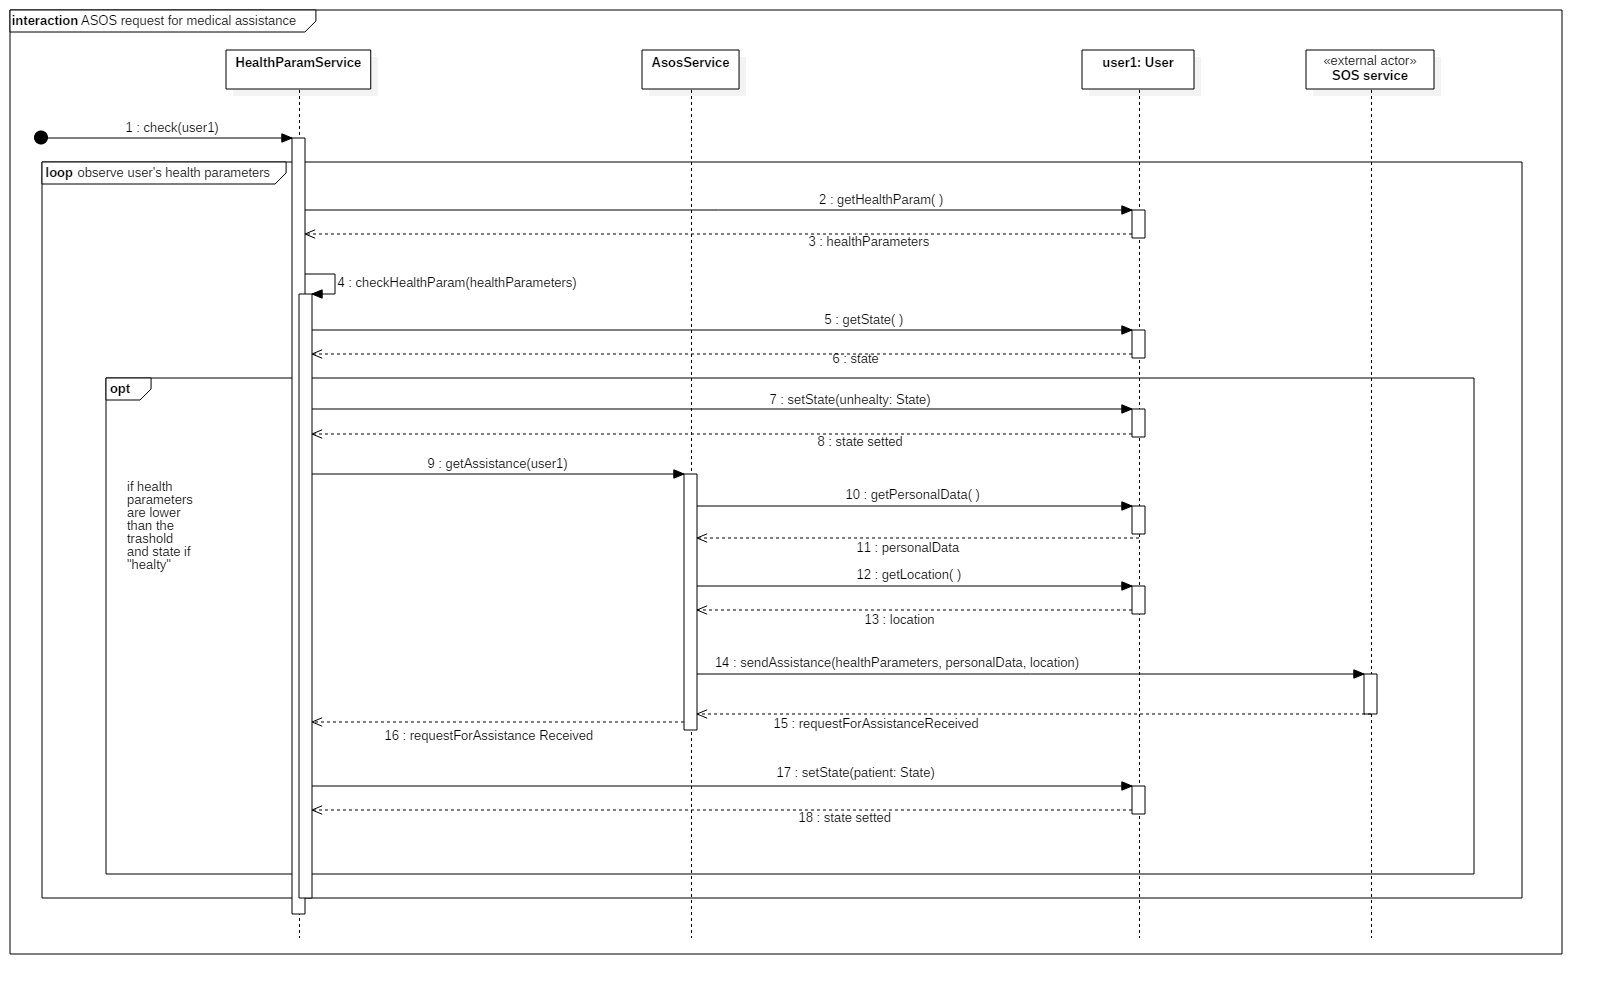
\includegraphics[width=1.0\textwidth]{./pictures/sequence_useAsos.png}\par
	\caption{Sequence diagram about ASOS requesting for assistance for a user.}
\end{figure}
\FloatBarrier 